\documentclass[12pt,openany]{report}
\usepackage[utf8]{inputenc}
\usepackage{graphicx}
\usepackage{hyperref}
\usepackage{biblatex}
\usepackage{listings,lstautogobble}
\usepackage{xcolor}
\usepackage{csquotes}
\usepackage{syntax}
\usepackage{framed}
\usepackage[skip=1pt]{caption} % example skip set to 2pt
\usepackage[section]{placeins}
\usepackage{textcomp}
\usepackage[htt]{hyphenat}
\usepackage{makecell}
\usepackage{lmodern}% http://ctan.org/pkg/lm
\usepackage{algorithm}% http://ctan.org/pkg/algorithms
\usepackage{algpseudocode}% http://ctan.org/pkg/algorithmicx}
\usepackage{forest}
\usepackage{multirow}
\usepackage{amsmath}

\usepackage{newfloat}
\DeclareFloatingEnvironment[
   fileext=lol,
   name=Listing
]{listing}
\DeclareCaptionSubType{listing}

 
\usepackage{subcaption}
\DeclareCaptionSubType{listing}

\definecolor{gray}{rgb}{0.4,0.4,0.4}
\definecolor{darkblue}{rgb}{0.0,0.0,0.6}
\definecolor{cyan}{rgb}{0.0,0.6,0.6}

\definecolor{pblue}{rgb}{0.13,0.13,1}
\definecolor{pgreen}{rgb}{0,0.5,0}
\definecolor{pred}{rgb}{0.9,0,0}
\definecolor{pgrey}{rgb}{0.46,0.45,0.48}

\graphicspath{ {images/} }
\addbibresource{references/*.bib}

\DeclareSourcemap{
  \maps[datatype=bibtex]{
    \map[overwrite]{
      \step[fieldsource=month, match=\regexp{\A(j|J)an(uary)?\Z}, replace=1]
      \step[fieldsource=month, match=\regexp{\A(f|F)eb(ruary)?\Z}, replace=2]
      \step[fieldsource=month, match=\regexp{\A(m|M)ar(ch)?\Z}, replace=3]
      \step[fieldsource=month, match=\regexp{\A(a|A)pr(il)?\Z}, replace=4]
      \step[fieldsource=month, match=\regexp{\A(m|M)ay\Z}, replace=5]
      \step[fieldsource=month, match=\regexp{\A(j|J)un(e)?\Z}, replace=6]
      \step[fieldsource=month, match=\regexp{\A(j|J)ul(y)?\Z}, replace=7]
      \step[fieldsource=month, match=\regexp{\A(a|A)ug(ust)?\Z}, replace=8]
      \step[fieldsource=month, match=\regexp{\A(s|S)ep(tember)?\Z}, replace=9]
      \step[fieldsource=month, match=\regexp{\A(o|O)ct(ober)?\Z}, replace=10]
      \step[fieldsource=month, match=\regexp{\A(n|N)ov(ember)?\Z}, replace=11]
      \step[fieldsource=month, match=\regexp{\A(d|D)ec(ember)?\Z}, replace=12]
    }
  }
}

\definecolor{comment}{RGB}{0,128,0} % dark green
\definecolor{string}{RGB}{255,0,0}  % red
\definecolor{keyword}{RGB}{0,0,255} % blue

\lstset{
  showspaces=false,
  showtabs=false,
  breaklines=true,
  showstringspaces=false,
  breakatwhitespace=true,
  basicstyle=\ttfamily,
  tabsize=2
}

\lstdefinestyle{codeStyle}{
  commentstyle=\color{pgreen},
  keywordstyle=\color{pblue},
  stringstyle=\color{pred},
  moredelim=[il][\textcolor{pgrey}]{$$},
  moredelim=[is][\textcolor{pgrey}]{\%\%}{\%\%}
}

\lstdefinelanguage{Jolie}{
  morekeywords={as,csets,type,configType,raw,any,undefined,void,default,
  if,for,while,spawn,foreach,else,define,main,include,from,
  constants,inputPort,outputPort,interface,execution,cset,
  nullProcess,RequestResponse,OneWay,throw,throws,install,
  scope,embedded,init,synchronized,global,is_defined,
  is_int,is_bool,is_long,is_string,bool,long,int,string,
  double,undef,with,location,protocol,interfaces,aggregates,courier,
  redirects,import,embed,service,binding,foreign,InputPort,OutputPort,implementation,private},
  morekeywords=[2]{>>,select,match},
  sensitive,%
	morecomment=[l]//,%
	morecomment=[s]{/*}{*/},%
	morestring=[b]",%
  morestring=[b]',%
  classoffset=1, % starting new class
  otherkeywords={;,|,@},
  classoffset=0% returning to previous class
}[keywords,comments,strings]%

\lstdefinelanguage{XML}
{
  morestring=[b]",
  morestring=[s]{>}{<},
  morecomment=[s]{<?}{?>},
  stringstyle=\color{black},
  identifierstyle=\color{darkblue},
  keywordstyle=\color{cyan},
  morekeywords={xmlns,version,type}% list your attributes here
}

\title{
{Jolie: Toward Production ready}\\
{\large University of Southern Denmark}\\
}

\author{
    Narongrit Unwerawattana\\
    Department of Mathematics and Computer Science\\
    \texttt{naunw18@student.sdu.dk}\vspace{40pt} \\
}
 
\begin{document}
\maketitle

\listoffigures
\listoftables


\chapter*{Introduction}

% introduction 
% ความเป็นมาและความสำคัญของปัญหา,จุดประสงค์,ขอบเขต,benefit ที่จะได้จากโปรเจคนี้

%idea 2 ---------------------
% ทำไมถึงมี SOC / Modular เพราะsoftware มีความเปน module?
% มีแล้วช่วยให้ software development ดีขึ้นยังไงลงดีเทลหน่อยนึง
% ด้วยประโยชน์ของภาษาที่รองรับ modular programmingจะช่วยให้การพัฒนาsoftware ดีขึ้นยังไง ยกตัวอย่าง
% ดังนั้นนี่จึงเป็นที่มาของ โปรเจคนี้โดยมีวัตถุประสงดังนี้ 
% บอกจุดประสงค์ ---> ศึกษาส่วนประกอบของภาษาโปรแกรมมิ่งที่รองรับ module system และพัฒนา Module system สำหรับภาษา Jolie 
% บอกขอบเขตของโปรเจคที่เราจะทำ(ของพี่แดนเขียนขอบเขตไว้ใน stucture of this thesis
% ของเราก็เขียนว่า feature อะไรบ้างที่เพิ่มเข้าไป
% ปิดท้ายด้วย benefit ที่จะได้จากการศึกษาและเพิ่ม feature ของ jolie

% What - why - how
% ทำไมถึงมี SOC / Modular เพราะsoftware มีความเปน module?


% เขียนแนวว่า ปัจจุบันอุสาหกรรม software มีความใหญ่และซับซ้อนขึ้น ได้มีการศึกษาถึงวิธีและ practical guideline and methodology to create a หนึ่งในวิธีการที่จะทำให้โค้ด maintain ได้ง่ายขึ้นคือการ ทำให้ system มีความเป็น modular โดยการ apply Seperation of concerns to plan and write code, 

For a long time, The demand for the principle and methodology of designing software has always been a point of discussion in software development.
As the software continuously evolved from time to time, Israeli et al. studied Linux kernel evolution for over 800 new versions and found that the size, from various metrics, has been increasing linearly from 1994 to 2008 \cite{10.1016/j.jss.2009.09.042}. Even for the present day, the development of the Linux kernel between 2019 to 2020, 1.3 million new lines of codes have been added to Linux kernel source code by 4,190 different contributors \cite{anderson2020}. For this reason, the goal of having straightforward, maintainable details in software, from an architectural point of view to the implementation level is crucial for every software development cycle.

The principle that is well known and adopted in many aspects of the related programming field is the Separation of Concerns (\textbf{SoC}). SoC aims to separate the problem into a small set of sub-problems to help the practitioner focus on one aspect, instead of being overwhelmed by the development complexity as a whole. Among many other principles, modularizing the system to smaller components is one of the prominent practices widely used in the industry.

\begin{displayquote}
    "the separation of concerns", which, even if not perfectly possible, is yet the only available technique for effective ordering of one's thoughts, that I know of. This is what I mean by "focussing one's attention upon some aspect"
    - Edsger W.Dijkstra\cite{dijkstra1974}
\end{displayquote}


The principle that is well known and adopted in many aspects of the related programming field is the Separation of Concerns (\textbf{SoC}). SoC aims to separate the problem into a small set of sub-problems to help the practitioner focus on one aspect, instead of being overwhelmed by the development complexity as a whole. Among many other principles, modularizing the system to smaller components is one of the prominent practices widely used in the industry.

Many software designs and principles adopt SoC as its fundamental principle to pursue an easy to maintain, interchangeable, and reusable software. From the architectural design point of view to the implementation detail aspect. From the very top level, Service-oriented architecture (\textbf{SOA}) focuses on the composition of services via communication over a network protocol. At the implementation level of software, modular programming is a design technique where the software is divided into several small, self-contain units, so-called a module. 

% // Service in SOA and Microservice
The SOA concept is well known for more than a decade, as it helped reduce the integration cost of information between services by providing a standard of data format. However, the developers and designers suffer from the complexity of implementing an SOA; one of the difficulties is the standard definition of the compositional protocol between services. Consequently, adopting the SOA concept has a trade-off between the integration cost as a business value and the additional cost of development. As we see, the beneficial organization for SOA, such as IT-related large companies or the business association, invested and experimented with the concept and published the definitions on their own\cite{cesar2020, ibmcloudeducation2019}.
% //https://opentravel.org/about-us/ 

The SOA system's complexity caused it to suffer from gaining technical maturity; thus, the attempt to rebrand SOA for the real-world application has resulted in the Microservice Architecture, which considered as an the second iteration of SOA \cite{Dragoni2017}. Microservice Architecture is a widespread software architectural paradigm whereby a service is defined as a standalone service, which means that it may not be composed of a combination of services. This definition reduces the complexity of implementing as it forces the designer to encapsulate only single business logic into a service, which makes the Microservice easier to implement and become a prominent software design at present. In recent years, it has become state-of-the-art software development, adopted by companies such as Amazon, Google, and Facebook.

Jolie\cite{JOLIE} is a service-oriented programming language that addresses the difficulty of developing a distributed system of services. Jolie tackles the difficulty of service implementation from the linguistic approach, unlike other general programming languages that usually require a combination of external technology building on top of each other to define a service. Jolie contributes a seamless experience for the developer in developing service as it provides the capability to define both communication method details and the workflow for the invocation operation.

The goal of this thesis is to develop a foundation of the module system for Jolie programming languages. We explore the design choices module system a develop one that is best-suited for Jolie's. We also have an experimental implementation of enhancement in Jolie type system to allow Jolie developer to define value constraints for a type. It is inspired by the work defining a schema for the JavaScript Object Notation (JSON)\footnote{JSON Schema https://json-schema.org/}, which is a well-known
data format used for communication between services in the present day.

The current work progress for Jolie Module System is partially merged into the Jolie the main development \url{https://github.com/jolie/jolie} repository is available at \url{https://github.com/kicito/jolie}.

% \section*{Structure of thesis}

This thesis structure as following
\begin{itemize}
    \item Chapter 1: discussion of the Module System and brief introduction of Jolie Programming Language
    \item Chapter 2: discussion of Jolie's Module system design space
    \item Chapter 3: description of Jolie's Module system implementation details
    \item Chapter 4: conclusion of this thesis
\end{itemize}
 
% % \section*{Notation used}

% \subsection*{Grammar}

% For this document, we use Extended Backus–Naur form (EBNF) notation to express the grammar of the programming language syntax. The following figure shows the example of grammar and the common syntax that will be used in the rest of this book 
% \begin{figure}[h!]
%     \begin{framed}
%         \begin{grammar}
%             <jolie> ::= <definitons>* <deployments>*  `main' `{' <behaviors> `}'

%             <definitons> ::= <typeDef> \alt \dots \alt <interfaceDef> 

%             <deployments> ::= \dots

%             <behaviors> ::= \dots
%         \end{grammar}
%     \end{framed}
%     \caption{An example grammar for Jolie}
% \end{figure}




% SOC เพื่อ ปูไปยัง Jolie
% Service-Oriented Computing (\textbf{SOC}) is a computing paradigm for developing an application by composing different services.
% Each of service defines it's own role and functionality in the application context\cite{papazoglou2003service}. 
% A service, or so called a program, proceeds it's execution by passing message from one to another. 
% The interest on \textbf{SOC} concept has been continuously gain attraction since \cite{JOLIE}.
% One of the research field related to \textbf{SOC} is the study of concurrency theory behind a process flow language, from it's specification of process by passing message, it can be formalizing the existing work flow language into message passing process calculus such as \(\pi\)-calculus.
% Similarly in industrial field, despite of missing the usage of term \textbf{SOC}, is focusing on the standardize the structured message; It is emphasized on constructing a seamless integration between service providers.

% Developing a service-oriented software had been criticized for being too constrained by the application it serve \cite{mckendrick_2009} \cite{SOA_opengroup}.
% This leads to an attempt to realizing the concept in the current state and implementation approach for \textbf{SOC}.
% The successful attempt of defining a modern service-oriented approach for develop a system is Microservice, where many of constrains has been relaxed in order to make implementation feasible for . 

% By using a set of expressive service based primitives. Jolie is also defined as a programming language for develop microservices as a code \cite{DBLP:journals/corr/GuidiLMM17}.  Jolie is 
% Supported modulesystem programming language

% intro to microservice
% Dragoni et al. studied and identified the history of the service-oriented architectural design and classified Microservice as a second iteration of an software design architecture that adopting \textbf{SOC} concept.
% Microservice has been exponentially gained it's popularity from since the term first coined in 2005 by Dr. Peter Rodgers, one of the major reason of Microservice success is due to the availability of tools and technology, this let development team in a company adopts the design pattern easily.

% SOA
% From the very top level, a software design style that embracing the modular design is called service-oriented architecture (\textbf{SOA}). \textbf{SOA} is a software architecture design that is focusing on the composition of services via a communication over a network protocol. The majority of \textbf{SOA} is implemented with Web Services technology, where services are composed together with the internet protocol such as SOAP, or HTTP. The implementation of \textbf{SOA} has been suffered by many difficulties mostly due to the following: lacking of tooling and testing framework \cite{vithanage_2014} \cite{JPM} and standard definition on the composition protocol between services. The latter reason had led to publication of several company owned definitions \cite{cesar2020} \cite{ibmcloudeducation2019}. \textbf{SOA} has contribute to a business value in many industry, it provides a standard of specification to ensure a seamless experience for connecting multiple systems together, for example, OpenTravel Alliance is an association by travel companies, which is focusing on develop a message structure for communication between global travel agency. It can be seen that majority of system that has adopt \textbf{SOA} is mostly a group of existing companies which shared the enterprise business context. From these reason has led to the difficulty on for a software architect to design a proper \textbf{SOA} style in a small system, and resulted in a problematic software with high technical dept.





% The early stage of \textbf{SOA} was focusing on defining a document format, in order to allow a service to be reuseable by different web service provider or

% maybe to background
% In \textbf{SOA}, A service is consist of four properties which are \cite{SOA_opengroup} :

% \begin{itemize}
%     \item a logical representation of a repeatable business activity that has a specified outcome
%     \item self-contained
%     \item may be composed of other services
%     \item a “black box” to consumers of the service
% \end{itemize}

% \textbf{SOA} is being reknown from 2005 from the rising of World-Wide web, where the emerging of web services has start to claim their interest from industry aspects. The \textbf{SOA} during those time was about working on definition of documents to be communicate with others to be able to query. this 

% The \textbf{SOA} had not initially got well received, due to it's complexity of the implementation and challenging of developing a testing framework \cite{vithanage_2014}.

% The top level of designing a software that applying this fundamental is called
% % collection of components defines a service, which usually responsible for a certain context in a business unit,


% With modular system, the program is analyzed and build up from bottom point of view; separating the concerns that has to be address in order to achieve the end product.

% Separation of concern

% It also helps reducing complexity on designing a system.

% Once it finished and get build up by composing as a whole.

% Separating of concerns has been develop in many aspects of development cycle, from the high level architectural design such as

% % what Module system for jolie
% Modular system, a system that built from composing a small unit so called module, has becoming a well adopted principle for

% Separation of concern is a

% A Modular program is a program that

% Sepa



% Modular programming is one of the key




% Jolie คืออะไร (ที่มา)
% % Microservice
% % เริ่มจาก SoC -> SOCK -> Jolie
% % มาจาก process calculi SOCK
% % Microservice is a programming practice that focusing on decomposing an application into small components which responsible for a single functionality for
% % 
% %  SOC
% Service-Oriented Computing (\textbf{SOC}) is a computing paradigm for developing an application by composing different services. Each of service defines it's own functionality and role in the application context\cite{papazoglou2003service}. A service, or so called a program, proceeds it's execution by passing message from one to another. The interest on \textbf{SOC} concept has been continuously gain attraction since \cite{JOLIE}. One of the research field related to \textbf{SOC} is the study of concurrency theory behind \textbf{SOC}'s workflow language, from it's specification of process by passing message, it can be formalizing the existing work flow language into message passing process calculus such as \(\pi\)-calculus. Similarly in industrial field, despite of missing the usage of term \textbf{SOC}, Dragoni et al. studied and identified Microservice as a second iteration of an software design architecture that adopting \textbf{SOC} concept. Microservice has been exponentially gained it's popularity from since the term first coined in 2005 by Dr. Peter Rodgers, one of the major reason of Microservice success is due to the availability of tools and technology, this let development team in a company adopts the design pattern easily.

% % SoA patterns chroreography and orchestration
% Approaches for designing a service-oriented application can be classified, by composition of services, in two patterns. The definitions of these two patterns have been developed from observing arts performance. The first approach, \textbf{choreography}, is the pattern where composition of service is done by considering as each of services perform their execution on it's own context, exposing an interfaces and it's location for others to connect. A service in choreography
% % A simple metaphor for describe this approach is considering a dancer who is performing their dance on a stage, without any leader, they perform their art by their self, only make a contract to other when the timing is right.
% On the other hand, \textbf{orchestration} is a pattern of centralizing the service's behavior by having a single service so call an orchestrator, coordinate and conduct a group of service to perform a task.

% % Jolie





% The concept of separating the concerns design principle has been mentioned on a published paper from   , the Service-oriented architecture (\textbf{SOA})


% % Modular Programming คืออะไร (ที่มา)
% % มีรูปแบบยังไง
% % ประโยชน์
% % ภาษาอะไรมีบ้าง
% % Module system
% Modular programming is one of the key component in modern programming languages. The emphasis of modularity is to separate functionality or concerns of a program to be an independent module such that it is self sufficient; it contains every information needed to perform a specific task.




% % Scope working importstatement for Jolie, alternate file Layout for jolie execution file
\tableofcontents
\chapter{Background}

\section{Jolie Programming Language}

\textbf{Jolie}\cite{JOLIE} is a general purpose programming language.
It is the first service-oriented programming language such that each of a a single Jolie program can be deployed independently as a service.
The goal of Jolie is to bring the formalized model of a service and composition calculus \textbf{SOCK} \cite{10.1007/11948148-27} and the practical workflow language WS-BPEL\cite{OASIS}.
For the syntax of language, Jolie use a block structured programming syntax similar to C and Java combined with effort to make the language simple and straightforward; as a result, learning curve for Jolie is flat for those who are already familiar with coding.

In this section, we briefly explain the Jolie program structure and it's components that are involved in Jolie module system. For those who keen to know more about advance topics in Jolie are recommended to visit \cite{joliedoc, JOLIE}.

Jolie program, or a service, is a file containing Jolie definitions which consists of three types of components, namely, the definitions, the service deployment description, and the service behavior.

Jolie definition declarations represent type structure definition and interface for a service.

A deployment description defines the communication layer of the service, such as protocol, location and the operation name accepted by a communication ports.

The detail of a service workflow is defined in service behavior part. The communication and computation instructions are composed together to a complex executable workflow which later will be execute at runtime.

Figure ~\ref{fig:JolieGrammar} demonstrate a syntax of Jolie program.

\begin{figure}[h]
    \begin{framed}
        \begin{grammar}
            <jolie> ::= <includeStmt>* <definition>* <deplInstruction>*  `main' `{' <behaviors> `}'
        \end{grammar}
    \end{framed}
    \caption{Jolie Program Syntax}
    \label{fig:JolieGrammar}
\end{figure}

\FloatBarrier

\subsection{Definition declaration}
\label{sec:jolie-def}

The definition declaration is a set of an information related to a service. The interface definition encapsulate operations into a group, which it is referred during defining a communication protocol. Each of the operation in Jolie is defined by a name and a message structure, or a type, required for passing and receiving. While the procedure definition groups instructions composition to be call in runtime execution. These declarations are used in the service itself, or can be defined in an external file and retrieved using include statement which is presented in section ~\ref{sec:jolie-include}.

\subsubsection{Type and Value Representation}
\label{sec:jolie-type-def}

Type system in Jolie is based on structural type system and is used to define the structure of message of send and receive messages. A type can be defined as a nested tree where each nodes contain value and it's children. Jolie support common primitive types with an additional two build-in types \textbf{raw} and \textbf{any}. The \textbf{raw} type is an internal type that is used for passing data and it cannot be created by the programmer. The \textbf{any} type indicates that the value can be in any form of the basic types. One of the key feature of jolie data storing is that every variable is storing a dynamic array.

As every variable in jolie is a dynamic array, cardinality can be define to ensure the range of occurrences for node in form of \textit{[ min, max ]} where min and max is a positive number indicate the range. The common quantifier shorthands such as ? and * is also support here. If cardinality is not defined, it will use default value of [1,1]. From this specification, an expression referring to a variable without an index is consider as referring to the value at its first index, as shown in the reference of \texttt{pet} field in figure ~\ref{fig:TypeDefinitonUsage}. 

The syntax of Jolie type definition grammar is shown in ~\ref{fig:TypeDefinitonSyntax} where \(<ID>\) is a name defined for it's type structure.

A type can be defined in three ways:
\begin{itemize}
	\item \texttt{typeInline} is a structural composition of types, as illustrated in Figure ~\ref{fig:TypeDefinitonUsage}.
	\item \texttt{typeLink} is a definition aliasing to a previously defined type.
	\item \texttt{typeChoice} is a type that can be represent from multiple types.
\end{itemize}

\begin{figure}
	\begin{framed}
		\begin{grammar}
			<typeDefinition> ::= `type' <ID> `:' <type>

			<type> ::= <typeInline>
			\alt <typeLink>
			\alt <typeChoices>

			<typeChoices> ::= <type> `|' <type>

			<typeLink> ::= <ID>

			<typeInline> ::= <nativeType> <subTypeBlock>?

			<subTypeBlock> ::= `{' `.'? <ID> <cardinality>? `:' <type>? `}'

			<cardinality> ::= `[' int `,' ( int | `*' ) `]'
			\alt `*'
			\alt `?'

			<nativeType> ::= 'void' | 'string' | 'raw' | 'any' | 'int' | 'double' | 'long' | 'bool'
		\end{grammar}
	\end{framed}
	\caption{Jolie Grammar\protect\footnotemark}
	\label{fig:TypeDefinitonSyntax}
\end{figure}

\footnotetext{ID denote an Identifier}

\begin{listing}
\begin{sublisting}{\linewidth}

\lstset{language=Jolie,
	style=codeStyle
}
\begin{lstlisting}[frame=tlrb, caption= {Constructing a type and value in Jolie}, label={list:type-value}]{typeDef-Jolie}
type person: int{
	name: void {
		firstname: string
		lastname: string
	}
	isMarried: bool
	pet[0, 2]: string
	age: int
}

person = 1
person.name.firstname = "John"
person.name.lastname = "Doe"
person.isMarried = false
person.pet = "Johnny"
person.pet[1] = "Max"
person.age = 20
\end{lstlisting}
\end{sublisting}\\[2ex]
\begin{sublisting}{\linewidth}
\lstset{language=XML,
showspaces=false
}
\begin{lstlisting}[frame=tlrb, caption= {XML representation of ~\ref{list:type-value}}, label={list:type-value-xml}]
<person>
	1
	<isMarried>false</isMarried>
	<name>
		<firstname>John</firstname>
		<lastname>Doe</lastname>
	</name>
	<pet>Johnny</pet>
	<pet>Max</pet>
	<age>20</age>
</person>
\end{lstlisting}
\end{sublisting}
\caption{ Jolie type Example }
\label{fig:TypeDefinitonUsage}
\end{listing}

\FloatBarrier

\subsubsection{Interface Definition}

The usage of Interface Definition in Jolie is to express a group of operations for the message passing communication. The operations in Jolie can be either a request-response type, or a one-way type. The type of operation defines an execution behavior of the service either to it is expected a message back from the server or not. The syntax for interface definition is shown in ~\ref{fig:InterfaceDefinitonSyntax}

\begin{figure}[h]
	\begin{framed}
		\begin{grammar}
			<interfaceDeclaration> ::= `interface' <ID> `{' ( oneWay | requestResponse ) `}'

			<oneWay> ::= (`oneWay' | `OneWay')  `:' <oneWayOp> ( `,' <oneWayOp> )*

			<requestResponse> ::= (`requestResponse' | `RequestResponse') \\ `:' <requestResponseOp> ( `,' <requestResponseOp> )*

			<oneWayOp> ::= <ID> `(' <type> `)' | <ID>

			<requestResponseOp> ::= <ID> `(' <type> `)' `(' <type> `)' <throws>? | <ID>

		\end{grammar}
	\end{framed}
	\caption{Jolie Interface Definition Syntax\protect\footnotemark}
	\label{fig:InterfaceDefinitonSyntax}
\end{figure}

\footnotetext{visit \cite{joliedoc} scope and fault section for an further information on fault handling}

By extending the type we had before, we can declare an interface as following
\begin{listing}[h]

\lstset{language=Jolie,
	style=codeStyle
}
\begin{lstlisting}[frame=tlrb]{typeDef-Jolie}
interface personInterface{
	requestResponse: createPerson(person)(bool)
	oneWay: createPersonAsync(person)
}
\end{lstlisting}
\caption{Jolie Interface declaration example}

\end{listing}

Here we define an interface of two operations, which required the passing message to be a structure of type `person". When invoking `createPerson" operation, the calling service will wait and expect a boolean value to be return from the target service to be execute. While `createPersonAsync' operation will just send the message and continue.

\FloatBarrier


\subsubsection{Procedure Definition}
\label{sec:jolie-procedure-def}

Jolie allows programmer to split process composition into a procedure, which can be invoked by calling the its name. Calling the procedure essentially tell the runtime execution to perform instruction within the caller scope. As an example at ~\ref{list:procedure}, calling \texttt{doubleX} in main scope cause \texttt{X} in the procedure to be referred to same \texttt{X} as the \texttt{main} scope. There are two types of special procedures in Jolie that define a target execution processes which are \texttt{init}, the initialization procedure, and \texttt{main}, the main execution target.

\begin{figure}[h]
	\begin{framed}
		\begin{grammar}
			<procedureDefinition> ::= `define' <ID> `{' <processes> `}'
		\end{grammar}
	\end{framed}
	\caption{Jolie Procedure Definition Syntax}
\end{figure}


\begin{listing}[h]
\lstset{language=Jolie,
	style=codeStyle
}
\begin{lstlisting}[frame=tlrb, caption= {Jolie procedure example}, label={list:procedure}]{procedure-Jolie}
define doubleX{
	X = X * 2
}

main {
	X = 5
	doubleX
	// now X == 10
}
\end{lstlisting}
\caption{Jolie procedure example}
\label{list:procedure}
\end{listing}

The \(<process>\) rule is the composition of tasks to be perform by the service, it will be discuss at \autoref{sec:jolie-behavior}.

\FloatBarrier


We can revisit the syntax of the \(<definition>\) rules as it can be represented by three components which are types, interfaces, and procedures as shown in figure ~\ref{fig:jolie-definition}

\begin{figure}[h]
    \begin{framed}
        \begin{grammar}
            <definition> ::= <typeDefinition>
            \alt <interfaceDeclaration>
            \alt <procedureDefinition>
        \end{grammar}
    \end{framed}
    \caption{Jolie Grammar for definition part}
    \label{fig:jolie-definition}
\end{figure}

\subsection{Deployment description}

Deployment description expresses the relation between services, whether it is a producer, consumer, or mediator of the interface.
These description is defined in a port which encapsulate details of communication specification in the system.
Jolie also provide a primitive to declare a dependency of the service, through embedding statement, which help Jolie programmer composing a complex service with ease.

\subsubsection{Communication Port}

The communication port is the only component needed to define a communication layer of the service.
It encapsulates detail needed to express a service, which are the listening protocol, location, and the interfaces. The location of port defines the communication channel for the port. For protocol part, Jolie supports a variety of communication protocols, not only limited to the web protocol like SOAP, HTTP and, SODEP (a Jolie specific binary protocol), it also supports the Bluetooth protocol and in-memory communication. Lastly, the interfaces define a list of operations related to the port depending on type of the port.

A Communication port in Jolie can be classified into two types, whether it is exposing a communication channel to the external service so called an \textit{inputPort}, or it is expressing the communication channel to other service, or the \textit{outputPort}.

Jolie also equipped with the primitives to define the advanced composition of the input port. One of the primitive that is offered by Jolie is \textit{aggregation}, which composes operations from a output port to defining input port and allows an input port to accept operations exposed in the output port. this allows developers to intercept a message between the two ports.

\begin{figure}[ht]
    \begin{framed}
        \begin{grammar}

            <outputPort> ::= `outputPort' \\ <portName> `{' <portConfigurationPair>+ `}'

            <inputPort>
            ::= `inputPort' <portName> `{' ( <portConfigurationPair> | <inputPortConfigurationPair> )+ `}'

            <portConfigurationPair>
            ::= `location' `:' \textit{StringLiteral}
            \alt `protocol' `:' <ID>
            \alt `interfaces' `:' <interfaceName>

            <inputPortConfigurationPair>
            ::=  `aggregates' `:' <portName> ( `,' <portName> )* \alt \dots

            <portName> ::= <ID>
            <interfaceName> ::= <ID>

        \end{grammar}
    \end{framed}
    \caption{Jolie Port Definition Syntax}
\end{figure}

\FloatBarrier

As an example of the concept presented in this section, we create a service as depicted in ~\ref{list:example-port-graphic}.
The service \texttt{program} acts as a producer of the operations in \texttt{personInterface}, where the communication channel is defined in \texttt{personInputPort}.
This service also acts as a consumer of \texttt{loggerInterface} defined by an output port \texttt{LoggerOutputPort}.
One key takeaway from this example is the usage of aggregation at line 11 which makes \texttt{personInputPort} accept the additional operations defined in \texttt{personInterface}. Different scenarios alter the behavior when an aggregated operation is invoked, for this specific example, since the operations in \texttt{loggerInterface} are distinct from the ones defined in the interface of the input port, Jolie will automatically forward the message to the origin aggregation output port.

For the interaction between ports through input/output operations, we will look at again in ~\ref{sec:jolie-behavior}.

\begin{figure}[ht]
    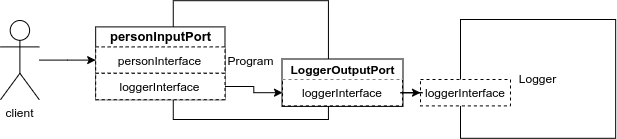
\includegraphics[width=10cm]{ExamplePort}
    \centering
    \caption{A service for port example}
    \label{list:example-port-graphic}
\end{figure}

\begin{listing}[ht]

    \lstset{language=Jolie,
        style=codeStyle,
        numbers=left,
        firstnumber=1
    }
    \begin{lstlisting}[frame=tlrb, caption= {Jolie Port declaration example}, label={list:example-port} ]{port-Jolie}
outputPort LoggerOutputPort {
    location: "socket://logger-service-location:3000"
    protocol: sodep
    interfaces: loggerInterface
}

inputPort personInputPort {
    location: "socket://localhost:3000"
    protocol: http
    interfaces: personInterface
    aggregates: Logger
}

main {
    createPerson(person)(result){
        log@LoggerOutputPort(person)
        result = true
    }
}
\end{lstlisting}
\end{listing}

In this section, we briefly show components for expressing a communication port in Jolie. Port can either be expressed as an incoming or outgoing communication. Both consist of fields that together define details for deploying a service, such as the operations and the message structure it accepts, the location it is using, and the communication protocol. Jolie is also equipped with a set of primitives that allow an advanced composition at the communication level, such as aggregation, which aggregates outgoing and incoming port, allowing the incoming port to accept and forward the message to the destination outgoing port.

\FloatBarrier


\subsubsection{Execution modality}

In the previous port decoration example at ~\ref{list:example-port}, the runtime execution terminates after service has finished the workflow of \texttt{createPerson} operation. But as a service, we would like the service to keep listening to the incoming messages without terminates after the first message has been processed.
Jolie offers a set of primitive of program execution behavior through \texttt{execution} statement which accepts three types of execution behaviors:

\begin{itemize}
    \item \textit{single}, a default behavior; which terminates the program after current process is finished.
    \item \textit{sequential}, initiate new execution behavior when the current process is finished.
    \item \textit{concurrent}, initiate new execution behavior whenever there is an operation invocation.
\end{itemize}

\begin{figure}[ht]
    \begin{framed}
        \begin{grammar}
            <executionMode>
            ::= `execution' `{' <modality> `}'

            <modality>
            ::= `single'
            \alt `concurrent'
            \alt `sequential'
        \end{grammar}
    \end{framed}
    \caption{Jolie Execution Modality Syntax}
\end{figure}

Thus, it is possible to change the service behavior in figure ~\ref{list:example-port} to accept multiple operations invocation concurrently by adding one single line of code as shown in line 5 of figure ~\ref{list:example-port-concurrent}

\begin{listing}[ht]

    \lstset{language=Jolie,
        style=codeStyle,
        numbers=left,
        firstnumber=1
    }
    \begin{lstlisting}[frame=tlrb, caption= {Jolie concurrent service example}, label={list:example-port-concurrent} ]{typeDef-Jolie}
outputPort LoggerOutputPort { ... }

inputPort personInputPort { ... }

execution {concurrent}

main {
    createPerson(person)(result){
        ...
    }
}
\end{lstlisting}
\end{listing}

\FloatBarrier

\subsubsection{Embedding Services}
\label{sec:embedded}

One of the service composition patterns widely uses is \textit{Orchestration}, which consist a central service, so-called an \say{orchestrator}, coordinates and conducts a group of services to achieve their responsibility together. The service orchestration can be achieved with ease by the embedding mechanism of Jolie; it allows multiple services to be executed in a single execution environment in a hierarchical order.
Moreover, it allows rapid communication of services via local memory communication, which delivers messages internally within the virtual machine.

The embedding mechanism expands a service into two roles, \textit{embedder} and \textit{embedded} service. The embedder conducts the services of the embedded. The mechanism allows the developer to separate a complex Jolie service into small single responsibility services that can later be reused in another project. 

The local memory communication channel can be defined by specifying a communication medium as \textit{local} in the \texttt{Location} field of the communication port.
Jolie offers a handy mechanism to embedded an external service into local execution.

Jolie supports different technologies to be embedded as a service, as it is not limited to a service defined in Jolie language. Currently, Jolie supports two additional services from external technology, which are Java and Javascript. Table ~\ref{table:embedded-technology-path} reports the list of supported technologies and the \(\langle path \rangle\) declaration a Jolie program must define to use the different supported technologies, as shown in table ~\ref{fig:embedded-syntax}

\begin{table}[h]
    \centering
    \begin{tabular}{ |c|l| }
        \hline
        Technology & Expecting content in path                                         \\
        \hline
        Jolie      & A path to a jolie file                                            \\
        Java       & A target to a java class which inherits Jolie's JavaService class \\
        Javascript & A path to a javascript file                                       \\
        \hline
    \end{tabular}
    \caption{Embedding technology and path content}
    \label{table:embedded-technology-path}
\end{table}


\begin{figure}[ht]
    \begin{framed}
        \begin{grammar}
            <embedStmt> ::= `embedded' `{' <embedTechnology> `:' ( <path> ( `in' <portName> )? )* `}'

            <embedTechnology> ::= 'Java' | 'Javascript' | 'Jolie';

            <path> ::= StringLiteral;

            <portName> ::= <ID>;

            <internalService>
            ::= 'service' <ServiceName> `{' processes `}';
        \end{grammar}
    \end{framed}
    \caption{Grammar for Jolie embedding statement}
    \label{fig:embedded-syntax}
\end{figure}

The syntax of \(\langle portName \rangle\) defined an output port name to be bound to the embedding service. There are three cases to be considered here, which is detailed in the list below:

\begin{itemize}
    \item If it is left blank, the embedding service will be launched as a standalone service.
    \item If it is pointing to an existing outputPort, the embedding service will bind a communication channel to the embedded service input ports declared \textit{`local'} in the location field.
    \item If it is pointing to a new outputPort, the embedding service will automatically create a new output port and bind communication channel to embedded service input ports declared \textit{`local'} in the location field.
\end{itemize}

The example in figure ~\ref{list:jolie-embeded} shows the usage of an embedded statement in Jolie. Here the communication protocol and the location at line 1 are not defined in code. It will be bound automatically to the communication port of embedded service before the main process starts to execute. 

\begin{listing}[ht]

\lstset{language=Jolie,
    style=codeStyle,
    numbers=left,
    firstnumber=1
}
\begin{lstlisting}[frame=tlrb]{typeDef-Jolie}
outputPort personService {
    interfaces: personInterface
}

embedded {
    Jolie: "person_service.ol" in personService
}

main {
    ... // person variable initialization omitted
    createPerson@personService(person)(result)
}
\end{lstlisting}
\caption{Jolie implementation of the embedded statement}
\label{list:jolie-embeded}
\end{listing}

\FloatBarrier



As before, we can now defines a syntax for the \(<deplInstruction>\) as following

\begin{figure}[h]
    \begin{framed}
        \begin{grammar}
            <deplInstruction> ::= <executionMode>
            \alt <outputPort>
            \alt <inputPort>
            \alt <embedStmt>
            \alt <internalService>
        \end{grammar}
    \end{framed}
    \caption{Jolie Grammar for deployment instruction part}
    \label{fig:jolie-depl}
\end{figure}


\subsection{Behavior declaration}
\label{sec:jolie-behavior}

The behaviors in Jolie define a composition of tasks, so called a processes, which is invoked when the service receive a message matching the exposed operation or when it is performing a sequential program. A process is essentially a program statement in other programming language, but as it is built from a distributed system concept, Jolie processes are composing in different way. Composing processes, as shown in the syntax rule \(<continuation>\) in figure ~\ref{fig:jolie-process}  uses semicolon \((;)\) to define a sequential statement and pipe \((|)\) for a parallel statement. For example given two statement \(A\) and \(B\) if we write \(A ; B\) Jolie interprets it as \textit{`execute A then B"} while \(A | B\) as \textit{`concurrently execute A and B"}. If the continuation is not defined, the default value is a sequential composition \((;)\).

In addition to the support of basic statements as other programming languages, Jolie natively supports a communication statements, which consist of two patterns, i.e. One-Way operation and Request-Response operation. As the name suggested, One-Way operation send a message through port and continue, while Request-Response waits for a response message from the target port then continue. With these concepts, a Jolie program encapsulate a whole communication procedure within a single statement. From the syntax, the \(<operationName>\), \(<outputPortName>\) are an identifier referring to the calling operation and port name respectively, while \(expr\) is an basic expression that is use to send and storing the received data.

Another service-oriented statement supported by Jolie is an Nondeterministic Choice defined in \(<ndInputChoices>\), which determine a workflow of the service, when the accepted operation get called. It is useful when a service is acting as provider in the system. The workflow consist of two parts of execution definition defined in \(<processes>\) syntax rule. Firstly, defined within square brackets scope, normally used for building an response for return to client since it is executing upon the operation is invoked. The second one, defined after the brackets, is performed after service has responded to the client, it useful in a situation where there are blocking tasks that do not contributed to the response message.

\begin{figure}[h]
    \begin{framed}
        \begin{grammar}
            <processes>
            ::= <process> ( continuation? <process> )*

            <continuation> ::= `|' \hfill (parallel composition)
            \alt `;' \hfill (sequential composition)

            <process> ::= \dots
            \alt <ndInputChoices> \hfill (non-deterministic Choice)
            \alt <inputStmt> \hfill (input operation statement)
            \alt <outputStmt> \hfill (output operation statement)

            <ndInputChoices>
            ::= <ndInputChoice>+

            <ndInputChoice>
            ::= '[' <inputStmt> `{' <processes> `}' ? ']' <processes>?

            <inputStmt>
            ::= <operationName> '(' <expr>? ')' \hfill (one-way)
            \alt
            <operationName> '(' <expr>? ')' '(' <expr>? ')' ( `{' <processes> `}' )? \hfill (request-response)

            <outputStmt>
            ::= <operationName> `@' <outputPortName> '(' <expr>? ')' \hfill (one-way)
            \alt
            <operationName> `@' <outputPortName> '(' <expr>? ')' '(' <expr>? ')' \hfill (request-response)
        \end{grammar}
    \end{framed}
    \caption{Jolie Grammar for deployment instruction part}
    \label{fig:jolie-process}
\end{figure}

Now lets look back to the Jolie service in example ~\ref{list:example-port}, at line 15-18

\begin{lstlisting}{ndChoice}
    createPerson(person)(result){
        log@LoggerOutputPort(person)
        result = true
    }
\end{lstlisting}
The statement \texttt{createPerson(person)(result)} tells the runtime execution to wait for a receiving operation \texttt{createPerson} and assign the receiving message to \texttt{person} variable then an execution proceed with the processes defined in brace scope. After the execution in the brace finished, the value in variable \texttt{result} will be sent back to the operation caller.


\FloatBarrier

\subsection{Include statement}
\label{sec:jolie-include}

Jolie support modular programming via an include statement. Similarly to C programming language include directive, when the parser found an include statement, it substitutes the statement into the content of the target input file. Include statement is used for separate file into a smaller component such as the interface definition file (.iol) or used for adding a functionality of the built in library. The include statement required a string literal indicating the location of the included file. If the given path is an absolute location, Jolie will attempt to find it directly. Otherwise, the searching paths are following.

\begin{itemize}
    \item A relative path resolved from the current working directory, where the jolie interpreter is called
    \item A relative path resolved from Jolie's standard \texttt{include} library directory.
    \item A relative path resolved from paths defined by the passing command line argument.
\end{itemize}

It is worth noting that the searching path is a relative path to the current working directory, not the program itself directory.

Jolie also supports code inclusion from the achieve files.
The including target string can specify as a Java JAR url like \texttt{<scheme>:file:<location>\newline!/{entry}} where \texttt{scheme} can be either a Java archive file (\texttt{jar}) or a Jolie achieve file (\texttt{jap}), \texttt{location} is a path to the archive file, and lastly \texttt{entry} is an internal path to a target inclusion file.

\begin{figure}[h]
    \begin{framed}
        \begin{grammar}
            <includeStmt> ::= `include' StringLiteral
        \end{grammar}
    \end{framed}
    \caption{Jolie Grammar for include statement}
    \label{fig:jolie-definition}
\end{figure}

\subsection{Jolie example program}

Once we are familiar with the basic concept of Jolie, we can demonstrate an example program of Jolie service, a sum service which take two integer and sum them together. We also going demonstrate how to invoke an operation of a service.

Firstly, the interface declaration file defined a list of shared definition between the client and sum service. which are type call \texttt{intPair} and the interface defining a operation that is used for communication.

\begin{listing}[ht]
    \lstset{language=Jolie,
        style=codeStyle
    }
    \begin{lstlisting}[frame=tlrb,caption={Sum service interface}, label={list:example-iol}]{sumIface.iol}
// sumIface.iol
type intPair: void{
    x : int
    y : int
}
interface SumIface{
    requestResponse: sum(intPair)(int)
}
\end{lstlisting}
\end{listing}

Then we define the sum server shown in figure ~\ref{list:example-sum}, which capable of performing a sum operation when it is called through an input port \texttt{IP}. In line 9 of server service, we instruct the service to execute a workflow instruction when receive an invocation. Lastly in our main behavior, we create a non deterministic choice as a handler for the operation defined in \texttt{SumIface}.

\begin{listing}
    \lstset{language=Jolie,
        style=codeStyle,
        numbers=left,
        firstnumber=1
    }
    \begin{lstlisting}[frame=tlrb, caption= {Sum service}, label={list:example-sum} ]{sumservice.ol}
include "sumIface.iol" // include interface file

inputPort IP{
    location:"socket://localhost:3000"
    protocol:sodep 
    interfaces:SumIface
}

execution { concurrent }

main{
    [sum(req)(res){
        res = req.x + req.y
    }]
}
\end{lstlisting}
\end{listing}

For our example of the service's client, we firstly include the standard library `console', which exposes us the ability to perform console related tasks eg. print and receive console input. Later at line 4 we declare a communication channel called \texttt{Calculator} which bind the communication channel to server's input port. Lastly we declare a behavior of the client, we basically build a message value and send it through invoke a operation \texttt{sum} in the output port.

\begin{listing}
    \lstset{language=Jolie,
        style=codeStyle,
        numbers=left,
        firstnumber=1
    }
    \begin{lstlisting}[frame=tlrb,caption= {Sum client example}, label={list:example-client}]{client.ol}
include "console.iol" // use build-in service "console"
include "sumIface.iol" // include an interface file 

outputPort Calculator{
    location:"socket://localhost:3000"
    protocol:sodep 
    interfaces:SumIface
}

define printResult{
    println@Console(result)()
}

main{
    req.x = 2;
    req.y = 3;
    sum@Calculator(req)(result)
    printResult
}
\end{lstlisting}
\end{listing}


\subsection{Jolie implementation}

In this section we will give an introduction to the implementation of Jolie programming language. After finished this chapter, the reader should follow the implementation design and changes that had made in Jolie internal implementation for support of the module system.

The implementation of Jolie language is based on interpretation approach. Therefore, the interpreter is responsible for total life-cycle of a Jolie program; parsing a program until executing it. There are four components that working together in order to interpret a Jolie program, a parser which parse source code into an Abstract Syntax Tree (AST), each Jolie behavior statement is later transform into a tree of Jolie executable process called OOIT (Object-oriented interpretation tree), the runtime environment which store the state and the responsible for executing the process, lastly, the Communication Core (CommCore) is the foundation of communication between Jolie runtime environment.

The workflow of interpreting a Jolie source code is following:

\begin{enumerate}
    \item The command-line configuration get parsed, this include locate the executing target file.
    \item The source code get parsed in parser, where the AST is created.
    \item The program's component nodes in AST get verified it's semantic. And resolve the type link definition
    \item The interpretation tree, or the runtime executable object, is generated from AST.
    \item The CommCore is initialized from the communication ports configuration declared in AST node.
    \item The embedding services is initialized and communication related variable is set.
    \item The runtime execute init/main procedure definition process.
\end{enumerate}

Type link definition is a definition that is referred to a type that is already defined. This may in a form of \lstinline{ type A : B } where B is a type definition previously defined in the program. The abstract syntax \texttt{A} gets resolved and linked to \texttt{B} during the verification of semantic in  

\FloatBarrier


%  parse configuration


\section{Module System}

Module system is a system consisting of composition of an independent executable program unit. A program unit contains every definition and functionality intended to solve one specific problem, each program unit is called Modules in the module system. Each module can be parsed into a module interface, which defines a name of public symbols and the required symbols from other modules. The module interface allows other modules access providing symbols and use its implementation details in their environment. The Module System targets the decomposition of large applications into smaller pieces. This led the developer of the supported module system programming language to reuse their codes and allow the concept of package managing tools, which helps engage its community to collaborate more and grow faster.

Import statement is the statement that is commonly used in the Modular programming language to access and retrieve definitions between modules. It is generally responsible for locating the target module, and resolve the definition to the local execution environment.

Usage of terms in the Module system varies between programming languages as their implementation detail of the module system. Before diving into the module's system of each selected popular programming language, the reader will be introduced with the term that is used within their context.

We had review the following programming languages such as

In the sections below, we mainly focus on Python programming language, since it's rich of documentation wise on it's history and their design choice available and it inspired our implementation of Jolie's module system.


\subsection{Python Module System}

The Python module system history and its design choices can be traced back to Modula-3\cite{modula-3}, as its modularity concepts influenced many modern programming languages, including Python.
Python acquired the Modula-3 usage of \texttt{dot} notation for traversing modules and elements\cite{python-foreward-essay}.

The Python's module system has been gradually evolving, in the years as shown in more than the 50 proposals related to the module system in Python Enhancement Proposals (PEP) \cite{pep0}. This chapter will discuss how Python 3.0 defined its module system and its importing mechanism.

A \textbf{module} is an object with a list of python definitions and executable statements. These statements are executed during the initialization of the module. In the file system perspective, a module is a file with 'py' extension, and the module is named after the file name.

A \textbf{package} is a module which might contain sub-modules or a sub-packages.
Thus, in the file system, directories are recognized as Python packages.
In the current version of Python, the packages are categorized into two types called regular packages and namespace packages.
A \textbf{regular package} is a package that is implemented as a directory containing \textbf{\_\_init\_\_.py} file.
The directory without a \textbf{\_\_init\_\_.py} is consider as a newer type package so-called \textbf{namespace package}.
The namespace package was introduced to natively support the declaration of a module from different locations \cite{pep420}. The element in the namespace package is called a portion, which can be a set of files in a single directory or an entry in a zip file.

\subsubsection{Import Statement}

Despite there exist a few methods for a module to invoke the import mechanism, we mainly focus on Python's import statement.
A dotted separate module name can specify the location of the target module. The target symbols are used to indicate symbol name in local namespace to be referred later for import statement caller or a wildcard character.
The syntax of import statements in Python is defined as follows in figure ~\ref{fig:python-import-stmt-syntax}.

\begin{figure}[ht]
    \begin{framed}
        \begin{grammar}
            <importStmt>
            ::= <importName>
            | <importFrom>

            <importName>
            ::= `import' <dottedAsNames>

            <importFrom>
            ::= `from' ( `.' )* ( <dottedName> | `.' ) `import' ( `*' | <importAsNames> )

            <importAsNames>
            ::= <importAsName> ( `,' <importAsName> )*

            <importAsName>
            ::= <NAME> ( `as' <NAME> )?

            <dottedAsNames>
            ::= <dottedAsName> ( `,' <dottedAsName> )*

            <dottedAsName>
            ::= <dottedName> ( `as' <NAME> )?

            <dottedName>
            ::= <NAME> ( `.' <NAME> )*

            <NAME> ::= <ID>
        \end{grammar}
    \end{framed}
    \caption{Python import statement syntax }
    \label{fig:python-import-stmt-syntax}
\end{figure}

An import statement of python has two forms, it is either in form of \texttt{<importName>} and \texttt{<importFrom>} statements. Both statements create identical instructions to the module importer, choice of use is subjectively open to the developer to pick. The semantics of these two forms is different from each other in the following way.

The first form of import, \texttt{<importName>}, every \texttt{<NAME>} declared in \texttt{<dottedName>} except the last one, must be a package, while the previous \texttt{<NAME>} can only be either a module or a package; it cannot be referred to a definition symbol inside a module.

For the second form, \texttt{<importFrom>}, the item element can be a module or any definition symbol declared within the package. In this form, it performs a lookup to symbol item inside the package; if not found, it continues with an attempt to import module items. The table ~\ref{table:python-import-def} shows the translation of symbols identified in a different form of import symbol.

\begin{table}[ht]
    \centering
    \begin{tabular}{ |l|p{0.7\linewidth}| }
        \hline
        Statement                   & Element explanation                                                                                                                                                 \\
        \hline
        import item                 & \textit{item} can either be a package or a module.                                                                                                                  \\
        \hline
        import item.subitem         & \textit{item} is a package while \textit{subitem} is a module in \textit{item}.                                                                                     \\
        \hline
        from pkg import item, item2 &
        \makecell[l]
        {If \textit{pkg} is a module,                                                                                                                                                                     \\ \textit{item} and \textit{item2} are definition symbols in \textit{pkg}                                                            \\
            If \textit{pkg} is a package,                                                                                                                                                                 \\ \textit{item} and \textit{item2} can either be a module in \textit{pkg} or \\ a definition defined in \textit{pkg}.
        }                                                                                                                                                                                                 \\
        \hline
        from pkg.mod import item    & \textit{pkg} is a package and mod is a module in \textit{pkg}, while \textit{item} can be a module of \textit{mod}, or a definition symbol defined in \textit{mod}. \\
        \hline
    \end{tabular}
    \caption{Python import element definition}
    \label{table:python-import-def}
\end{table}

There are two types of import statement in Python which determine the module lookup location \cite{pep328}. Absolute import is the default behavior for an import statement, where it will perform a lookup based on the list of system module lookup path. Other types of import statements, relative import, instruct the system to perform a lookup for module relatively from the module that an import statement resides.

A useful feature that \texttt{<importFrom>} provides to Python developer is an ability to specified a module target location. If the module target is prefixed with a dot (.), it will be considered a relative import, where a dot serves as go one level up.


\subsubsection{Import Mechanism}

After the import statement's execution is completed, it results to a set of defined definitions ready to use in the caller's execution context.
To achieve this goal, Python processes import statement in two steps, during the creation of symbol table, which the importing target symbols are created the global execution scope of the import statement caller, then the runtime execution of it combines the search of the named module and the binding of the result to the importing module's symbol reference.

At the implementation level, these two operations are performed by an abstraction called \texttt{importer}, which consists of two other crucial abstraction objects: finders and loaders.
Finders are responsible for performing module lookup, while loaders use the result from the finder to execute and create a module object which later is saved to the cache.
Lastly, the loader binds names as defined in the import statement to the local execution environment.

Python locates a module with a \texttt{finder}, which is categorized into two types based on the location where the finder should attempt to find the module.
Firstly the \texttt{MetaPathFinder} will perform a lookup on a list of paths passing through the finding method.
The second type of finder, the \texttt{PathEntryFinder}, performs a look-up only on at a list of paths to the path that is assigned during its creation.
Searching operations may cause certain side-effects to the execution environment. In case of importing a module inside the package, it is processed by importing each parent packages from top-level until the module is reached, which means it also executes the initialization instructions of every module target's parent packages.

After the module has been loaded into the execution environment, the importing target symbols are binding to the importer global execution scope; this scope is also called the module scope. There is only a single global scope in the Python program execution.

\subsubsection{Symbol Privacy}

In Python, every declaration of the symbol is considered a private symbol if it having a prefixed underscore (\_). Such a symbol will be ignored for a wildcard import (from ... import *), and an error will be raised when it is implicitly referred to, as the declaration can only be used in its module scope.


\chapter{Jolie Module System}

\section{Definitions}

Before diving into the details, it is useful to define a definition of components in a module system. In Jolie,
\begin{itemize}
    \item
          A \b{symbol} is a declaration of file level definition AST node. Symbol target is defined along with a module target in the import statement to specify which definition node it to be imported.
    \item
          A \b{module} is defined as a Jolie execution code in the file system. A module is a file contains symbols and the execution target for running the jolie code.
    \item
          A \b{package} is defined as either a directory in the file system or a  file. A package role in the jolie module system is a place to hold the modules and can be part of the module target.
\end{itemize}


% วิธีการพัฒนา
% algorithm
\subsection{Experimental Design: Refinement type}

In this chapter, we discuss an experimental feature of the refinement type. We believe that it has potential on the module system for defining a constrain on the type system. The current implementation is not accepted feature to the Jolie main repository, but it is available at https://github.com/kicito/jolie/tree/jolie-module-3.

Tchitchigin et al. studied refinement Type of Jolie to implement a dynamic and static type checking for Jolie native type with the type verification done by the SMT solver \cite{DBLP:journals/corr/TchitchiginSMEM16}. The study resulted in the reduction of the testing effort and enhanced the security of the service.

In our implementation, inspired by the JSON Schema\footnote{JSON Schema https://json-schema.org/}, extends Jolie type system to support the creation of a value format for each field, we also added a capability to define a default value for a service parameter. Whenever the value is missing during type validation, instead of raising an error, the default value will get assigned, and the execution proceeds.

The syntax of the declaration of type is defined as follows.

\begin{figure}[ht]
    \begin{framed}
        \begin{grammar}
            <refinedType> ::= `type' <ID> `:' <type>  '(' refinedTypeRule ( ',' refinedTypeRule)* ')'
            
            <refinedTypeRule> ::= rulename '(' ruleArg ( ',' ruleArg )* ')'
            
            <ruleArg> ::= expression | refinedTypeRule
            
            <typename> ::= ID
            
            <rulename> ::= ID
        \end{grammar}
    \end{framed}
    \caption{Jolie Refinement Syntax}
    \label{fig:JolieRefinementGrammar}
\end{figure}

The syntax of refined type is extended from the existing type syntax, a set of type rules defined within the parenthesis after the type construction. Within the \textit{refineTypeRule}, two specifiers of \textit{rulename} it's expression is defined. The \textit{rulename} is a set of available predicates for the specific type. The following table describes the available predicate for each Jolie native type.

\begin{figure}[ht]
    \begin{tabular}{ |l|l|l| }
        \hline
        Type    & Predicate                                            & Description                   \\
        \hline
        boolean & default(x)                                           & is_defined(value) ? value : x \\
        \hline
        \multirow{5}{4em}{number}
                & default(x)                                           & is_defined(value) ? value : x \\
                & minimum(x)                                           & value $\ge$ x                 \\
                & exclusiveMinimum(x)                                  & value $>$ x                   \\
                & maximum(x)                                           & value $\le$ x                 \\
                & exclusiveMaximum(x)                                  & value $<$ x                   \\
        \hline
        \multirow{4}{4em}{string}
                & default(x)                                           & is_defined(value) ? value : x \\
                & minLength(x)                                         & value $\ge$ x                 \\
                & maxLength(x)                                         & value $\le$ x                 \\
                & pattern(x) \footnotesize{where x is an regex expression} & x.match(value)                \\
        \hline
    \end{tabular}
    \caption{Jolie refinement type rules}
    \label{fig:jolie-refinement-rules}
\end{figure}

With this simple yet powerful set of predicates available in refinement type, the developer is capable of defining a value constraint and control the possible value of the receiving parameter as shown in the example below of the \textit{twiceService} ~\ref{fig:jolie-refinement-example}.

\begin{listing}[ht]
    \lstset{language=Jolie,
        style=codeStyle,
        numbers=left,
        firstnumber=1
    }
    \begin{lstlisting}[frame=tlrb,
basicstyle=\footnotesize]{refinement-type-service.ol}
interface twiceIface{
    RequestResponse: twice(int)(int)
}

type twiceParam: void{
    .location: string(
        pattern(^socket:\/\/localhost:3000$)
    )
    .protocol: string(default("sodep"))
}

service twiceService(param : twiceParam){
    inputPort myPort{
        location: param.location
        protocol: param.protocol
        interfaces: twiceIface
    }

    main{
        twice(req)(res){
            res = req * 2
        }
    }
}
\end{lstlisting}
    \caption{Jolie example service for refinement type}
    \label{fig:jolie-refinement-example}
\end{listing}

Here, we defined \textit{twiceService}, which accepts a value of type \textit{twiceParam}; the received value is later used as a configuration of the incoming communication port \textit{myPort}. The refinement type of \textit{location} and \textit{protocol} are specify in the way that the service developer of \textit{twiceService} can assure that the received value from client it match the predicate given in type declaration.

Refinement type is a practical and powerful feature that could be a research topic in the further development of Jolie. As we are seeing, the refinement type gives service owner authority to determine and limited possible information from the embedder service. Yet, with this specification, it also introduces the uncertainty of execution behavior for Jolie type checking and may yield an unexpected result; for example, given a list of condition predicate and the default rule, what is the proper execution order of predicate checking. One other crucial case is the method to determine that the rules have no conflict. For these reasons,  further study on the Type Refinement could be an interesting topic that could enhance the experience of developing a Jolie service in the future.

% \chapter{Appendix}

\printbibliography

\end{document}
